\documentclass[a4paper,10pt]{article}
%\usepackage[latin1]{inputenc} % Paquetes de idioma
\usepackage[utf8]{inputenc} % Paquetes de idioma (Este encoding toma acentos :) )
\usepackage[spanish]{babel} % Paquetes de idioma
\usepackage{graphicx} % Paquete para ingresar gráficos
\usepackage{grffile}
\usepackage{hyperref}
\usepackage{fancybox}
\usepackage{amsmath}
\usepackage{amsfonts}
\usepackage{listings}
\usepackage{float}
% Paquetes de macros de Circuitos
%\usepackage{pstricks}
\usepackage{tikz}

% Encabezado y Pié de página
\usepackage{fancyhdr} % Paquete para encabezados y pie de página
\pagestyle{fancy} % Sin esta línea no se imprimiría el encabezado en todas las páginas

\fancyhf{} %  Borra el encabezado anterior (Por defecto escribe el títutlo de la sección en la que se encuentra la hoja
\setlength{\headheight}{22.55pt}
\fancyhead[L]{
	{\textsf{Facultad de Ingenier\'ia $-$ Universidad de Buenos Aires \\ 66.44 Instrumentos Electrónicos}}
}
%\addtocounter{page}{5}
\fancyhead[R]{\thepage}

\renewcommand{\footrulewidth}{0.4pt} % Ajusta el tamaño de las líneas separadoras en el pié de página
\renewcommand{\headrulewidth}{0.4pt} % Ajusta el tamaño de las líneas separadoras en el encabezado

\fancyfoot[L]{
	{\textsf{Trabajo Pr\'actico N$^{\circ}4$}: Mediciones de impedancias} \\
	{\textsf{Integrantes: Eduardo Sanchez, Francisco Soler}}
	}
		

% Carátula del Trabajo
\title{ \author{} % Lo pongo para que el warning no moleste :p
\setlength{\unitlength}{1cm} %  Especifica la unidad de trabajo
\thispagestyle{empty}

\begin{picture}(18,0)
\put(0,0){
\includegraphics[width=1.5cm, height=3cm]{Logo1.png}}

\put(10.5,0){
\includegraphics[width=3cm, height=3cm]{Logo2.png}}

\end{picture}
\\[1.5cm]
\begin{center}
	\textbf{{\Huge Facultad de Ingenier\'ia \\ Universidad de Buenos Aires}}\\[2cm]
	{66.44 Instrumentos Electrónicos}\\[0.5cm]
	{Trabajo Pr\'actico N$^{\circ}3$: Mediciones de impedancias}\\[2.5cm]
\end{center}

\begin{flushleft}
	\textbf{Integrantes:} \\[1cm]

	\begin{tabular}{|c|c|c|}
		\hline
		\textbf{\normalsize Padr\'on} & \textbf{\normalsize Nombre} & \textbf{\normalsize Email} \\
		\hline
		\normalsize 92903 & \normalsize Sanchez, Eduardo Hugo & \normalsize hugo\_044@hotmail.com \\
		\hline
		\normalsize 91227 & \normalsize Soler, Jos\'e Francisco & \normalsize francisco.\_tw@hotmail.com \\
		\hline
		\normalsize xxx & \normalsize Wawrynczak, Claudio  & \normalsize claudiozak@gmail.com \\
		\hline
	\end{tabular}
\end{flushleft}
\date{} % Hace que no se imprima la fecha en la cual se compilo el .tex
 }

\begin{document}
	\maketitle % Hace que el título anterior sea el principal del documento
	\newpage

	\tableofcontents % Esta línea genera un indice a partir de las secciones y 
					 % subsecciones creadas en el documento
	\newpage


	\section{Objetivo}
	
	\indent	El objetivo de este trabajo pr\'actico consiste en conocer el funcionamiento del analizador de espectro y mostrar algunos de sus m\'ultiples usos posibles.
	
	\newpage
	\section{Introducci\'on}
	Un analizador de espectro es b\'asicamente un instrumento que permite visualizar la composici\'on espectral de frecuencias de una se\~nal de entrada. Un diagrama en bloques simplificado puede observarse en la Figura \ref{diagramadebloques}. En la Figura se puede observar que la se\~nal de entrada pasa inicialmente por un atenuador y por un filtro pasabajos (cuyo uso determina sin ambig\"uedad el rango de frecuencias con las que se opera, aunque si se lo elimina permite extender el rango de frecuencias del analizador ). Luego pasa a un multiplicador donde se multiplica con la se\~nal generada por un oscilador local estable. A la salida del multiplicador se encuentran se\~nales cuyas frecuencias son sumas y diferencias de las frecuencias del oscilador local y de la se\~nal de entrada. Las componentes m\'as relevantes se encuentran en $f=f_{osc}-f_{\text{se\~nal}}$ y $f=f_{osc}+f_{\text{se\~nal}}$, pero en general, cuando se utiliza el filtro pasabajo de entrada la componente que interesa es solamente $f=f_{osc}-f_{\text{se\~nal}}$.
	Si alguna de estas se\~nales producidas tiene la frecuencia del filtro pasabanda intermedio, $f_{IF}$, \'esta es luego amplificada logar\'itmicamente (la escala generalmente utilizada en pantalla es en decibeles), rectificada por un detector de envolvente, filtrada por un filtro de video y es utilizada para establecer la se\~nal vertical de la pantalla.
	Con respecto al eje horizontal (el de frecuencias), un generador de rampa controla su barrido de izquierda a derecha. A su vez este mismo generador se encarga de controlar la frecuencia del oscilador local, la cual var\'ia proporcionalmente con la tensi\'on de la rampa. De esta forma se pueden barrer las frecuencias presentes en la se\~nal de entrada y mostrarlas en pantalla.
	\begin{figure}[!htb]
					\centering
					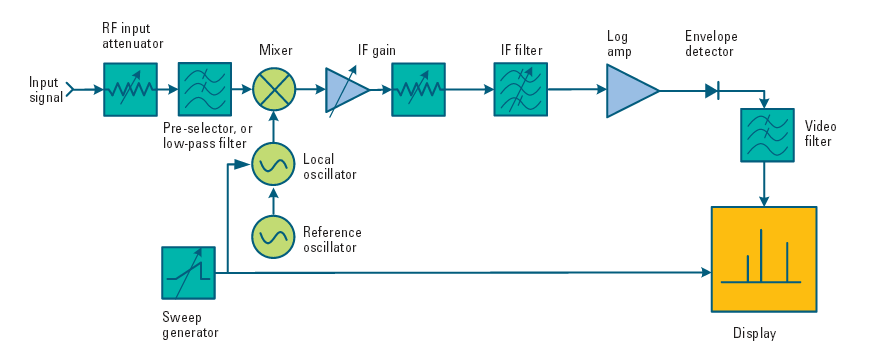
\includegraphics[width=12cm]
					{Imagenes/diagram.PNG}
					\caption{Diagrama en bloques de un analizador de espectro superheterodino}
					\label{diagramadebloques} 
			\end{figure}
	\newpage
	\section{Desarrollo}
\indent Para llevar a cabo las mediciones, se utilizan los siguientes
		instrumentos:
		\begin{itemize}
			\item Analizador de espectro HM 5006
			\item Analizador de espectro LPT 6000
			\item Generador de funciones Agilent N9310A
			\item Cable coaxil para conexi\'on de los instrumentos
		\end{itemize}	
		%HUGO
		\subsection{Selectividad}
		La resoluci\'on en frecuencia de un analizador de espectro es su capacidad para poder distinguir 2 se\~nales senoidales de la misma amplitud. Este valor se especifica como el ancho de banda de los filtros FI cuando su respuesta cae $3~dB$. 
		Sin embargo, si las se\~nales es\'an separadas en la frecuencia de resoluci\'on pero con diferente amplitud puede ocurrir que una quede enmascarada dentro de la otra. De esta manera surge otra especificaci\'on que es la selectividad, la cual se define como la relaci\'on entre el ancho de banda cuando la respuesta cae $60~dB$ y cuando cae $3~dB$. Matem\'aticamente 
		$$S=\frac{BW(-60~dB)}{BW(-3~dB)}$$
	
		En esta secci\'on se obtiene la selectividad de los analizadores de espectro HM5006 y PSA 6000 con diferentes resoluciones. Para ello se conectan por medio de un cable coaxil a un generador Agilent N9310A que produce un se\~nal senoidal. En la Tabla \ref{selectividad} se puede observar los resultados obtenidos.
		
		\begin{table}[!htp]
			\centering
			\begin{tabular}{|c|c|c|c|c|}
				\hline
				Analizador & Resoluci\'on & $BW(-60~dB)$ & $BW(-30~dB)$ & Selectividad \\
				\hline
				$13.3~MHz~\pm1.5\%$& $25~pF~\pm0.1pF$& $182~\pm7\%$ & 
				$5.73~\mu Hy~\pm3.40\%$ &$ 2.63~\Omega~\pm8.5\%$ \\
				\hline
				$10.7~MHz~\pm1.5\%$& $40~pF~\pm0.1pF$& $200~\pm7\%$ & 
				$5.54~\mu Hy~\pm3.25\%$ &$ 1.86~\Omega~\pm8.5\%$ \\
				\hline
				$9.6~MHz~\pm1.5\%$& $50~pF~\pm0.1pF$& $200~\pm7\%$ & 
				$5.50~\mu Hy~\pm3.20\%$ &$ 1.66~\Omega~\pm8.5\%$ \\
				\hline  
				$6.9~MHz~\pm1.5\%$& $100~pF~\pm0.1pF$& $195~\pm7\%$ & 
				$5.33~\mu Hy~\pm3.10\%$ &$ 1.18~\Omega~\pm8.5\%$ \\
				\hline  										 	  	  
			\end{tabular}
			\caption{Mediciones con el Q-metro} \label{selectividad}
		\end{table}	
		%HUGO. Me encanta la THD 
		\subsection{Distorsi\'on arm\'onica de un generador de funciones}
				\indent En la Figura \ref{img001}
				\begin{figure}[!htb]
						\centering
						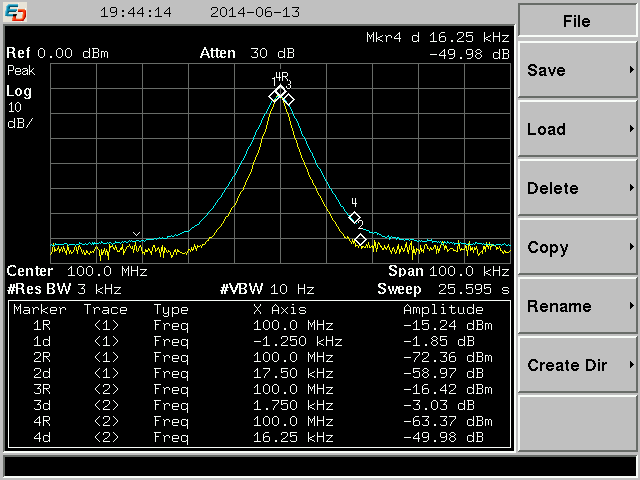
\includegraphics[width=8cm]
						{Imagenes/SCREN443.PNG}
						\caption{Medici\'on para la resistencia de $10k\Omega$. La 
						referencia (en blanco) esta graficada con la l\'inea abierta.}
						\label{img001} 
				\end{figure}
		%No esntendi mucho lo de la distorsi�n por. FRAN?			
		\subsection{Distorsi\'on por intermodulaci\'on del analizador de espectro}
		\subsection{Frecuencia de conversi\'on de un generador digital}
		%HUGO. Creeo que entendi lo de ruido de fase
		\subsection{Ruido de fase}
		\subsection{Modulaci\'on AM}
		%HUGO. Las funciones de Bessel de FM son para mi jeje
		\subsection{Modulaci\'on FM}
		\subsection{Figura de ruido}
	\section{Conclusiones}
	\indent
\end{document}

